\chapter{Variables}
\label{ch:variables}
\section{Introduction}

\begin{tcolorbox}[title=Goal]
\textbf{Practice} creating and updating Python variables, use basic operators and comparisons on one Iris flower sample, and build the stable variable names that later sessions will reuse.
\end{tcolorbox}

\begin{tcolorbox}[title=You will work in]
Use the following file for this session:
\begin{itemize}
    \item \texttt{session2/session2\_iris\_template.py} (main student file)
\end{itemize}
\textbf{How to run the file:} Always run this script from the project root using the terminal command: \\
\texttt{python3 session2/session2\_iris\_template.py} \\
\textbf{Do not edit other files.}
\end{tcolorbox}

\noindent
This is \textbf{Session \ref{ch:variables}} of the course.
This lab session starts our \textbf{one-dataset journey}: the \textbf{Iris dataset}.
From session 2 until session 12, we will consistently use Iris only, while building programming skills step-by-step until we can build and compare simple classifiers. Programming becomes easier when you are comfortable changing values and observing outputs. Your goal for this session is to practice changing flower measurements and seeing how derived values and comparisons change.

\begin{tcolorbox}[title=Hands-on file for this session]
Work only in the following file:
\begin{itemize}
    \item \texttt{session2/session2\_iris\_template.py}
\end{itemize}
\textbf{How to run the file:} Use \texttt{python3} in the integrated terminal or click the Run button in VS Code. \textbf{Do not edit other files.}
\end{tcolorbox}

\begin{figure}[H]
    \centering
    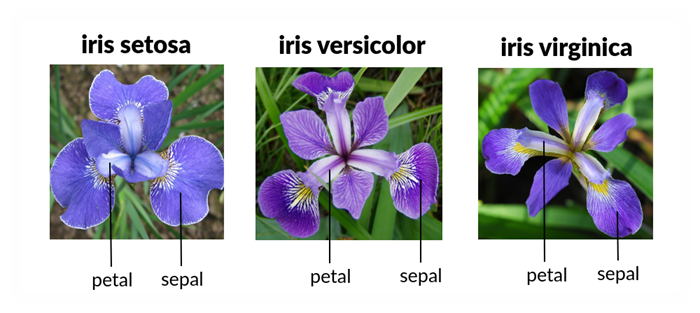
\includegraphics[width=0.85\textwidth]{session2/image/differenty_types_iris.png}
    \caption{Session 2 focus on Iris fundamentals (image extracted from \href{https://miro.medium.com/v2/resize:fit:1100/format:webp/1*uo6VfVH87jRjMZWVdwq3Vw.png}{miro.medium.Com}).}
\end{figure}

\section{What You Will Learn}

For today (session 2), we are not doing machine learning yet.
Instead, we treat one Iris flower as normal 

Python variables so you can practice:
Upon completing this tutorial, you will be able to:

\begin{enumerate}
    \item Declare clear variable names for one Iris sample,
    \item Compute a derived value with operators,
    \item Use a comparison that returns \texttt{True}/\texttt{False},
    \item Print your student label for submission,
    \item Define stable variable names reused in Sessions 3-5.
\end{enumerate}

\section{Canonical Variables}

It is imperative to use consistent variable names across sessions. We enforce these names so next session's template can reuse your variables without changes. Therefore, we will familiarize you with the canonical variable names for Iris samples and rule settings.

\begin{itemize}
    \item Sample fields: \texttt{id}, \texttt{sepal\_length}, \texttt{sepal\_width}, \texttt{petal\_length}, \texttt{petal\_width}, \texttt{species}
    \item Rule settings: \texttt{threshold}, \texttt{feature\_name}, \texttt{positive\_label}, \texttt{negative\_label}, \texttt{label\_key}
\end{itemize}

\section{Iris Dataset Background}

The Iris flower dataset (often called Fisher's Iris dataset) is a classic multivariate dataset introduced by the statistician and biologist Ronald Fisher in his 1936 paper on using multiple measurements in taxonomic problems. It contains sepal and petal measurements for three Iris species and underpins many foundational examples in linear discriminant analysis. This material serves as the single dataset we will reuse throughout the course, so a solid grasp of its structure accelerates every subsequent session.

\section{Flower Features and Data Types}

Each Iris flower (and any other object we might study) has observable characteristics such as color, sepal width, petal length, or even the species label itself. In data analysis these characteristics are called \textbf{features}. When we write code, each feature is stored inside a \textbf{variable}. So when you see a programming variable like \texttt{sepal\_length}, you can think of it as the code representation of a real-world feature.

Variables are not all the same: each one stores a specific data type. For example, lengths and widths are usually \texttt{float} values because they can contain decimals, while labels such as the species name are \texttt{string}s. Keeping track of data types helps avoid bugs and makes later calculations easier. The table below lists the canonical variables you will manipulate throughout the Iris exercises along with their typical data types.

\begin{table}[H]
    \centering
    \begin{tabular}{|p{0.35\textwidth}|p{0.2\textwidth}|p{0.35\textwidth}|}
        \hline
        \textbf{Variable / Feature} & \textbf{Data Type} & \textbf{What it represents} \\
        \hline
        \texttt{id} & string & Unique identifier for the flower sample \\
        \texttt{sepal\_length} & float & Sepal length measurement in centimeters \\
        \texttt{sepal\_width} & float & Sepal width measurement in centimeters \\
        \texttt{petal\_length} & float & Petal length measurement in centimeters \\
        \texttt{petal\_width} & float & Petal width measurement in centimeters \\
        \texttt{species} & string & Class label such as \texttt{setosa} or \texttt{virginica} \\
        \texttt{feature\_vector} & list of floats & Ordered measurements (e.g., [sepal, petal values]) \\
        \texttt{threshold} & float & Rule cutoff when comparing a measurement \\
        \texttt{feature\_name} & string & Name of the feature the rule evaluates \\
        \texttt{positive\_label} & string & Label to assign when the condition is true \\
        \texttt{negative\_label} & string & Label to assign when the condition is false \\
        \texttt{label\_key} & string & Dictionary key used to store the chosen label \\
        \hline
    \end{tabular}
    \caption{Canonical Iris variables and the data types we will use in code.}
\end{table}

This provides a structured way to store and access various attributes of the flower, including:

\begin{enumerate}
    \item \textbf{Flower Identity:} A unique identifier for the sample (\texttt{id}).
    \item \textbf{Sepal Measurements:} \texttt{sepal\_length} and \texttt{sepal\_width}.
    \item \textbf{Petal Measurements:} \texttt{petal\_length} and \texttt{petal\_width}.
    \item \textbf{Species Label:} The class name for the sample (\texttt{species}).
    \item \textbf{Feature Vector:} A compact list of numeric values (\texttt{feature\_vector}) used for quick processing.
\end{enumerate}


%%%%%
\section{Starter: One flower as variables}

\noindent
\begin{tcolorbox}[title=Task 1: Print Flower Summary]
Run the script \texttt{session2/session2\_iris\_template.py}. 
\end{tcolorbox}

Open the file named \texttt{session2/session2\_iris\_template.py}. 
Run the script by clicking the Green "Run" button at the top-right corner in VS Code.The Run button looks like a green triangle (similar to a play button in media players) as shown in \ref{img:run_button}. When you click it, VS Code will execute the Python script and display the output in the terminal below.

\begin{figure}
    \centering
    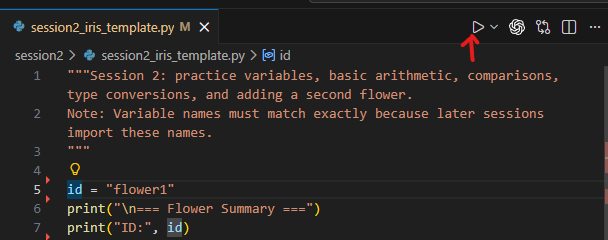
\includegraphics[width=0.8\textwidth]{session2/image/run_button.png}
    \caption{Green "Run" button in VS Code to execute the Python script.}
    \label{img:run_button}
\end{figure}

You should see a printed summary of the flower's ID in the terminal.

You should see the output as below:
\begin{lstlisting}[language=Python]
=== Flower Summary ===
ID: flower1
\end{lstlisting}

The terminal is located at the bottom of your VS Code window. If you don't see it, you can open it by going to the menu and selecting \texttt{View > Terminal} or using the shortcut \texttt{Ctrl + `} (Windows) or \texttt{Cmd + `} (Mac).
The terminal should look like in the image \ref{img:terminal}.
\begin{figure}[H]
    \centering
    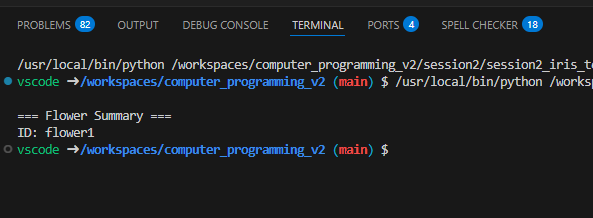
\includegraphics[width=0.8\textwidth]{session2/image/terminal_output.png}
    \caption{Example terminal output after running the starter Iris script.}
    \label{img:terminal}
\end{figure}

\subsection{Experimenting with different Iris values}

\noindent
\begin{tcolorbox}[title=Task 2: Change this to "flower\_2x]
Change the value of the \texttt{id} variable from \texttt{"flower1"} to \texttt{"flower\_2x"}.
\end{tcolorbox}


As mentioned above, programming becomes easier when you are comfortable changing values and observing outputs.
Your goal for this session is to practice changing flower Id.

First, try changing the flower ID value from \texttt{id = "flower1"} to \texttt{id = "flower\_2x"} in the code.
Run the script again and observe the output.

You should see:
\begin{lstlisting}[language=Python]
=== Flower Summary ===
ID: flower_2x
\end{lstlisting}

\begin{tcolorbox}[title=Checkpoint]
You should see \texttt{ID: flower\_2x}.
\end{tcolorbox}
\begin{tcolorbox}[title=Common Mistakes]
If you get an error, check if you accidentally removed the quotes around the string or misspelled the variable name.
\end{tcolorbox}

Great! You have successfully modified the flower ID variable.
Now, just to ensure you are comfortable with changing values, try changing the flower ID to any other string you like (e.g., \texttt{"my\_flower"}, \texttt{"iris\_sample\_01"}, etc.).
Run the script again and observe the output.
You should see the updated flower ID in the output as below:
\begin{lstlisting}[language=Python]
=== Flower Summary ===
ID: my_flower
\end{lstlisting}

Now, change it back to \texttt{"flower1"} for the next tasks.

\subsection{One Iris Flower as Variables}

\noindent
\begin{tcolorbox}[title=Task 3: Define more variables for one Iris flower]
Decomment some of the lines by removing the symbol $\#$ at the beginning of line and, change the variable values to represent the measurements and species of the flower as described in the instructions.
\end{tcolorbox}


Now that you have practiced changing the flower ID, let's add more variables to represent the flower's measurements and species. In the Python template, some of the variables are already defined for you. You just need to fill in the values.
\begin{itemize}
    \item Let's set the \texttt{id} flower to \texttt{"flower1"}.
    \item Then, we set the \texttt{sepal\_length} equal to \texttt{5.1} (float).
    \item Next, we set the \texttt{sepal\_width} equal to \texttt{3.5} (float).
    \item Then, we set the \texttt{petal\_length} equal to \texttt{1.4} (float).
    \item Next, we set the \texttt{petal\_width} equal to \texttt{0.2} (float).
    \item Finally, we set the \texttt{species} equal to \texttt{"setosa"} (string).
\end{itemize}

Then, when you run the script, you should see the full flower summary printed as below:
\begin{lstlisting}[language=Python]
=== Flower Summary ===
ID: flower1
Sepal Length: 5.1
Sepal Width: 3.5
Petal Length: 1.4
Petal Width: 0.2
Species: setosa
\end{lstlisting}

\begin{tcolorbox}[title=Checkpoint]
You should see the 6 attributes printed cleanly without errors.
\end{tcolorbox}
\begin{tcolorbox}[title=Common Mistakes]
Check your variable names exactly: \texttt{sepal\_length} not \texttt{sepal\_lenght}.
\end{tcolorbox}

\section{Derived Variable with Operators}

\begin{tcolorbox}[title=Task 4: Compute petal area]
Place the variable {petal\_length} and \texttt{petal\_width}, but multiply them together to compute the petal area and store it in a new variable named \texttt{petal\_area}. 
\end{tcolorbox}


As we discussed in the lecture, you can compute new values using existing variables and operators.
For example, you can compute the petal area by multiplying \texttt{petal\_length} and \texttt{petal\_width}.
Add the following line to your code to compute \texttt{petal\_area}:
\begin{minted}[fontsize=\small, linenos, frame=lines]{python}
petal_area = petal_length * petal_width
\end{minted}

\subsection{Your Task: Compute Petal Area}
Before you run the script, uncomment the print statement for petal area in the flower summary section, or else it will not show in the output. There are two ways to uncomment:
\begin{itemize}
    \item Remove the \texttt{\#} symbol at the start of the line that prints petal area.
    \item Or, if you are using VS Code, you can highlight the line and press \texttt{Ctrl + /} (Windows) or \texttt{Cmd + /} (Mac) to toggle commenting.
\end{itemize}

When you run the script again, you should see the petal area printed as below:
\begin{lstlisting}[language=Python]
Petal Area: 0.28000000000000003
\end{lstlisting}

\begin{tcolorbox}[title=Checkpoint]
You should see a floating-point number representing the area.
\end{tcolorbox}
\begin{tcolorbox}[title=Common Mistakes]
If nothing prints, ensure you properly uncommented the line and you don't have indentation errors.
\end{tcolorbox}

\section{Comparison Result}
\subsection{Introduce Stable Rule Variables}

Next session (session 3), we will build a simple rule-based classifier. This mimics simple screening rules used in biology or triage systems!
A common beginner rule for Iris is:

If the petal length is less than 2.0 cm, classify the flower as "setosa"; otherwise, classify it as "not\_setosa".

In mathematical notation, this can be expressed as:

\[
    \text{if } petal\_length < 2.0 \Rightarrow \text{"setosa"}, \text{ else "not\_setosa"}
\]

To prepare for this, we will define stable variable names for the rule settings.

\subsubsection{Create a threshold variable}
\begin{enumerate}
    \item Create a variable \texttt{threshold} with value \texttt{2.0}.
    \item Compare \texttt{petal\_length} with \texttt{threshold}.
    \item Print the boolean result.
\end{enumerate}

Define these values exactly:
\begin{minted}[fontsize=\small, linenos, frame=lines]{python}
threshold = 2.0
feature_name = "petal_length"
positive_label = "setosa"
negative_label = "not_setosa"
label_key = "species"
\end{minted}

These variables are preparation for Session 3 classifier logic.

\noindent
Try different \texttt{petal\_length} values and observe how \texttt{True/False} changes.

\subsection{Task 4: Comparison Result (No if-statement yet)}

\begin{tcolorbox}[title=Task 5: Comparing with threshold]
Create a boolean variable \texttt{is\_short\_petal} that checks if \texttt{petal\_length} is less than \texttt{threshold}. 
\end{tcolorbox}


Create and print:
\begin{minted}[fontsize=\small, linenos, frame=lines]{python}
is_short_petal = petal_length < threshold
\end{minted}

This gives a boolean output and prepares you for Session 3 conditionals.

\begin{tcolorbox}[title=Checkpoint]
You should see \texttt{True} for the setosa sample since 1.4 < 2.0.
\end{tcolorbox}

% \section{Type Conversion Practice}

% In real programs, you often read values as strings (for example, from a file).
% We will practice conversions safely.

% \subsection{Task 5: Type Conversion Practice}
% Practice string-number conversion:
% \begin{minted}[fontsize=\small, linenos, frame=lines]{python}
% petal_length_text = str(petal_length)
% threshold_text = "2.0"
% threshold_number = float(threshold_text)
% \end{minted}

% Print each value with \texttt{type(...)}.

% \subsubsection{Your Task: Show conversions}
% \begin{enumerate}
%     \item Create \texttt{petal\_length\_text} using \texttt{str(petal\_length)}.
%     \item Create \texttt{threshold\_text} using \texttt{"2.0"} (a string).
%     \item Convert it into a float using \texttt{float(threshold\_text)}.
%     \item Print the values and their types using \texttt{type()}.
% \end{enumerate}

% \begin{lstlisting}[language=Python]
% print("\n=== Conversions ===")
% \end{lstlisting}

% \begin{tcolorbox}[title=Checkpoint]
% You should see type outputs such as \texttt{<class 'str'>} and \texttt{<class 'float'>}.
% \end{tcolorbox}

\section{Take Home Exercise: Add a Second Flower with \_2 Suffix}

You are tasked to create a second flower based on the \textit{Iris setosa} shown in the image below. 
Define the variables with the measurements (sepal length, sepal width, petal length, and petal width) exactly as displayed in the figure. 
To avoid confusion with the variables from the previous tasks, append the suffix \texttt{\_2} to each variable name (e.g., \texttt{sepal\_length\_2}, \texttt{species\_2}). This suffixing ensures we can convert them correctly in Session 3.

\begin{figure}[H]
    \centering
    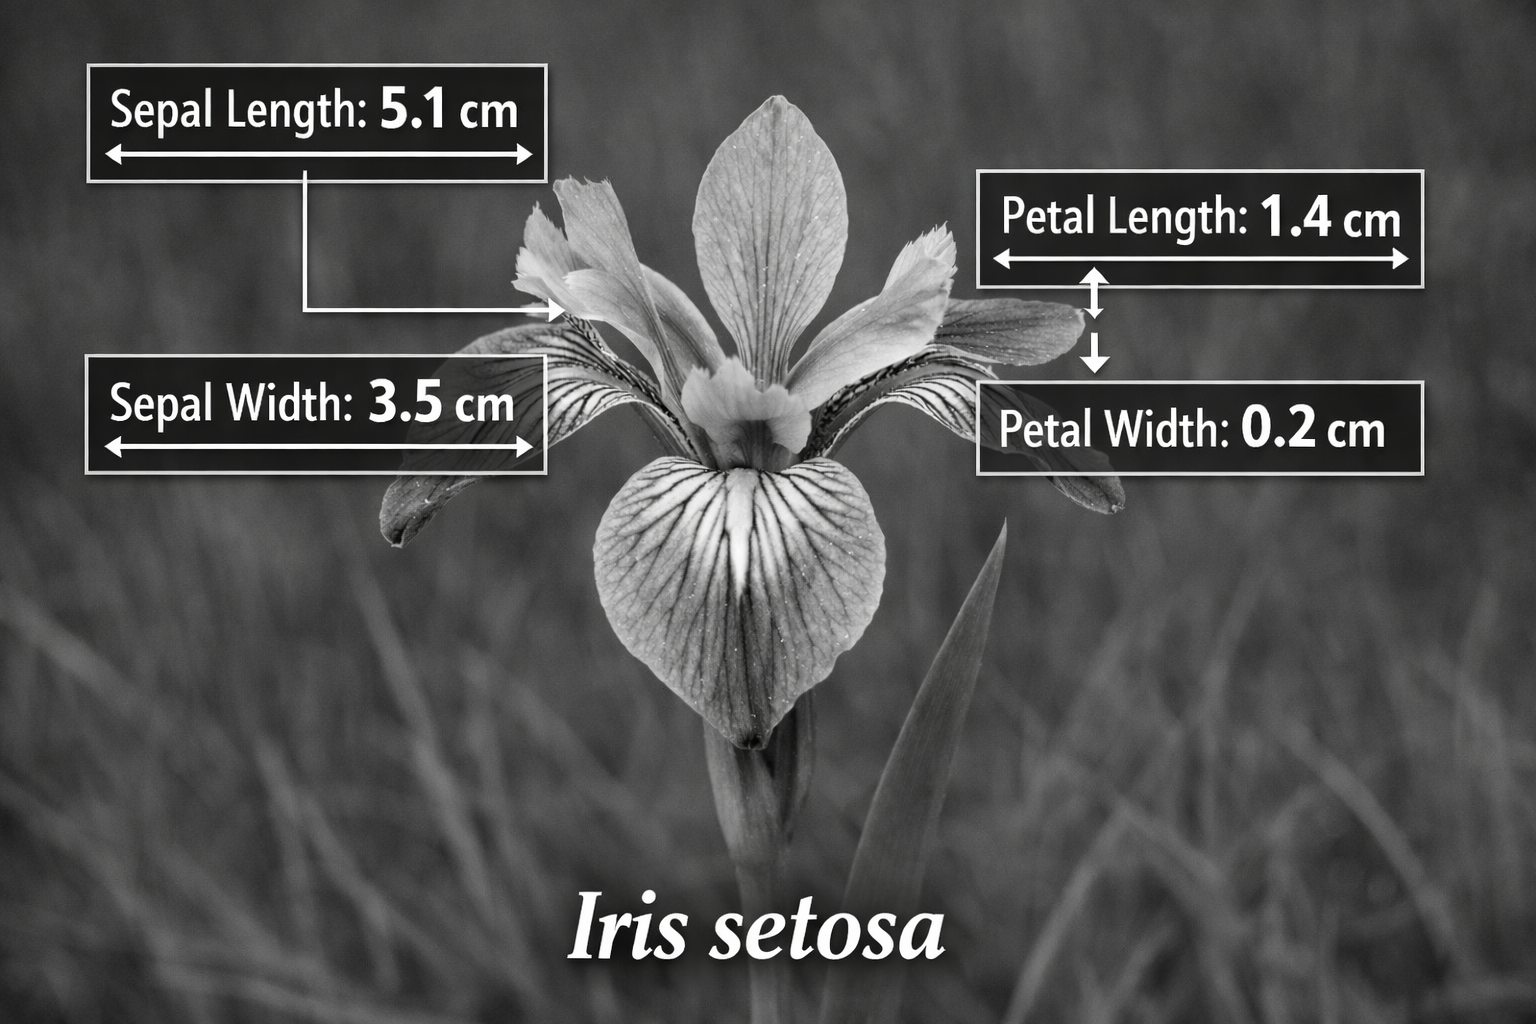
\includegraphics[width=0.5\textwidth]{session2/image/iris_setosa.png}
    \caption{Iris setosa flower with sepal length, sepal width, petal length, and petal width with measurement as shown in the image (image artificially generated).}
\end{figure}

Your specific tasks are:
\begin{enumerate}
    \item Define the variables: \texttt{sepal\_length\_2}, \texttt{sepal\_width\_2}, \texttt{petal\_length\_2}, \texttt{petal\_width\_2}, and \texttt{species\_2}.
    \item Assign the values visible in the image to these variables.
    \item Compute the petal area for this second flower and store it in a variable named \texttt{petal\_area\_2}.
    \item Print the calculated area.
\end{enumerate}

\begin{minted}[fontsize=\small, linenos, frame=lines]{python}
# Example of the computation (ensure you define the variables first!)
petal_area_2 = petal_length_2 * petal_width_2
print(petal_area_2)
\end{minted}

\begin{tcolorbox}[title=Hint]
Use the measurements shown in the figure to define \texttt{sepal\_length\_2}, \texttt{sepal\_width\_2}, \texttt{petal\_length\_2}, \texttt{petal\_width\_2}, \texttt{species\_2}. Make sure the expected output matches what you did for the first flower.
\end{tcolorbox}

\begin{tcolorbox}[title=Checkpoint]
Ensure you get the right \texttt{petal\_area\_2} by multiplying 1.4 by 0.2.
\end{tcolorbox}

\begin{lectureronly}
    \textbf{Solution Notes for Task 6:}
    Instructor values: 
    \texttt{sepal\_length\_2 = 4.9}, \texttt{sepal\_width\_2 = 3.0}, \texttt{petal\_length\_2 = 1.4}, \texttt{petal\_width\_2 = 0.2}, \texttt{species\_2 = "setosa"}.
\end{lectureronly}

\section{Expected Output When Submitting in Itel}

In the terminal, you should see the following output when running the program:
\begin{minted}[fontsize=\small, linenos, breaklines=true, frame=lines]{python}
=== Flower Summary ===
ID: flower1

=== Flower Summary ===
ID: flower1
Sepal Length: 5.1
Sepal Width: 3.5
Petal Length: 1.4
Petal Width: 0.2
Species: setosa

Petal Area: 0.27999999999999997

=== Comparison ===
is_short_petal (petal_length < threshold): True

=== Conversions ===
petal_length_text: 1.4 | type: <class 'str'>
threshold_text: 2.0 | type: <class 'str'>
threshold_number: 2.0 | type: <class 'float'>

=== Flower 2 ===
Petal Area 2: 0.27999999999999997
\end{minted}


\section{Summary \& Review}
\begin{itemize}
    \item \textbf{Variables:} You defined variables to store flower features.
    \item \textbf{Data Types:} You converted data between strings and floats.
    \item \textbf{Operators:} You derived new variables using basic arithmetic.
    \item \textbf{Comparisons:} You practiced boolean expressions for rule checks.
\end{itemize}

\textbf{Review Questions:}
\begin{enumerate}
    \item What happens if you set \texttt{petal\_length = 3.0} in the comparison task?
    \item Why do we use floats for length but strings for species?
    \item What is the difference between \texttt{2.0} and \texttt{"2.0"} in Python?
\end{enumerate}

\textbf{Micro-Exercise:} Change the \texttt{threshold} variable to \texttt{1.0} and predict what the \texttt{is\_short\_petal} output will be before running it!
